\documentclass[review=true, screen, acmlarge]{acmart}
\settopmatter{printacmref=false} % Removes citation information below abstract
\renewcommand\footnotetextcopyrightpermission[1]{} % removes footnote with conference info
\setcopyright{none}
\pagestyle{plain} % remove running headers

\usepackage{booktabs} % For formal tables
\usepackage[utf8]{inputenc} %use utf-8 to enable german (and other non-ascii) character encodings
\usepackage{csquotes} % for quotes / blockquotes


%\usepackage[ruled]{algorithm2e} % For algorithms
%\renewcommand{\algorithmcfname}{ALGORITHM}
%\SetAlFnt{\small}
%\SetAlCapFnt{\small}
%\SetAlCapNameFnt{\small}
%\SetAlCapHSkip{0pt}
%\IncMargin{-\parindent}


% Document starts
\begin{document}
% Title portion
\title{CTNDCI: Identifying the Challenges Towards a distributed Nano Data Center Infrastructure} 

\author{Melanie Hauser}
\affiliation{%
  \institution{LMU Munich}
  \city{Munich} 
  \country{Germany}}
\email{melanie.hauser@campus.lmu.de}

\author{Diana Irmscher}
\affiliation{%
  \institution{LMU Munich}
  \city{Munich} 
  \country{Germany}}
\email{d.irmscher@campus.lmu.de}

\author{Katrin Kolb}
\affiliation{%
  \institution{LMU Munich}
  \city{Munich} 
  \country{Germany}}
\email{katrin.kolb@campus.lmu.de}

\author{Mengchu Li} 
\affiliation{%
  \institution{LMU Munich}
  \city{Munich} 
  \country{Germany}}
\email{mengchu.li@yahoo.com}

\author{Katharina Rupp}
\affiliation{%
  \institution{LMU Munich}
  \city{Munich} 
  \country{Germany}}
\email{katharina.rupp@web.de}

\author{Andreas Scholz}
\affiliation{%
  \institution{LMU Munich}
  \city{Munich} 
  \country{Germany}}
\email{andreas.scholz@campus.lmu.de}




\begin{abstract}
In this paper we identify the challenges currently preventing nano data centers from becoming the dominant form of content provision on the internet. With the global increase in IP traffic the question of how to provide and deliver data is becoming increasingly important. Monolithic data centers, as they are used today, pose several problems, such as high energy consumption and lack of scalability. An alternative solution mitigating the problems of monolithic data centers has been proposed in the form of a distributed nano data center infrastructure. Research has shown this to be a superior solution. However, no widespread solution based on a nano data center infrastructure has been implemented as of yet. By identifying the main challenges nano data centers are facing steps can be taken to overcome these challenges in a more focused way, leading to a more economic data distribution.\\



\end{abstract}


\keywords{Green IT; Nano data center; Energy consumption; Security; Availability; Scalability; Data distribution}

\maketitle


\section{Introduction}
Nowadays, concerns about the environment are increasing and finding alternatives that reduce waste, CO2-emission or energy consumption, is a challenging topic. In order to fight environmental problems, it is essential that sustainable solutions are realized in every possible area. These areas also include internet content provision and storage.\\ Traditionally, monolithic data centers are used to store and manage today's constantly rising mass of data. This centralized approach, though, consumes huge amounts of energy and especially cooling is a severe issue. To overcome these issues and provide a more energy-efficient approach, de-centralized models have been introduced. Among others, the model of nano data centers was advocated. This kind of data center solution is said to be highly energy-efficient while still providing sufficient content availability and uptime.\\ 
Thus, the question arises why no such approach has been realized so far. Also, the media attention towards the topic is quite low, even so the findings presented in the according papers, which will be treated in section \ref{StateOfTheArt}, are very promising. \\
Therefore, the purpose of this paper is to identify challenges that prevent the large-scale realization of nano data centers: 
\begin{itemize}
\item What are political and legal challenges that yet have to be overcome?
\item What are technical challenges that have yet to be overcome, especially:
\begin{itemize} 
\item Are nano data centers really as energy efficient as the previous papers indicate? 
\item If so, are the energy savings as high for all use cases? 
\end{itemize}
\end{itemize}
These questions will be answered in the course of this paper. To achieve this, scientific publications concerning nano data centers, as well as related approaches were researched and compared. Moreover, an interview was conducted with an expert on monolithic data centers, to gain further insight into data center models and real world problems that might not yet have come up or seemed relevant in theory.\\
At first, related papers are presented. After that, the used methodology is described and challenges towards a distributed nano data center infrastructure are discussed. The challenges extracted from relevant papers rise from a variety of categories. In this paper, though, only political, legal and technical challenges are analysed in depth. After presenting our findings, we will evaluate and discuss them. Lastly we provide an outlook on what future work could be done to help with the decision process of whether nano data centers are a realistic future alternative to monolithic data centers.


% Head 1
\section{State of the art}
\label{StateOfTheArt}
Many researchers have already mentioned some challenges regarding nano data centers. Still, they focus more on the positive aspects of them rather than explaining these challenges. For this reason this paper is focusing on identifying these challenges in more detail. In this section, the state of the art on the current research on nano data centers is presented. 
\subsection{ECHOS}
ECHOS introduces a concept for Nano Data Centers that can or should completely replace monolithic data centers \cite{Laoutaris:2008:EEC:1341431.1341442}. The authors call it a radical solution for data management and provision.
According to this concept, so-called "boxes" are set up at the edges of the network, eg. in home gateways (see \cite{technicolor}). These boxes communicate with each other via a peer-to-peer system. The peer-to-peer system as well as the bandwidth is controlled by a central unit, such as the ISP. However, the approach of networking boxes via a peer-to-peer system, and thus providing or sharing content, requires some conditions. So it is first necessary to provide a distributed hosting edge infrastructure. Furthermore, there are also some other problems mentioned. In ECHOS these are listed as follows \cite{Laoutaris:2008:EEC:1341431.1341442}:
\begin{itemize}
	\item "Lack of service guarantees due to uncontrolled interface between different applications."
	\item "Inefficient use of network's and other peer's resources and consequently suboptimal performance."
	\item "Even if sufficient status information is in place, still P2P is inherently unable to use it as it was designed around selfish user behavior and free-riding prevention mechanism [...]."
	\item "Absence of security and control make it impossible to guarantee the integrity and security of content."
\end{itemize}
The problems here are only superficially addressed, and accordingly the solutions to the problems are more general. In this thesis it is conveyed that it is very easy to develop a nano data center platform. The solutions are rather unsatisfactory, and require more investigations.
\subsection{NaDa}
In the paper from Valancius et al. \cite{DBLP:conf/conext/ValanciusLMDR09} another Nano Data Center approach called NaDa is proposed. Based on a variant of a peer-to-peer network, NaDa consists of distributed servers managed and controlled by an ISP. According to the authors, devices like DSL or Cable modems can serve as gateways and replace monolithic data centers regarding the use of many Internet services. Their papar, though, only covers video streaming services. 

The authors claim that NaDa consumes up to 30\% less energy than a traditional data center in this use case. The following challenges can be extracted from the paper:

\begin{itemize}
	\item The ISP needs to invest into gateways with more storage and bandwidth to create a reliable network.
	\item There is no research into other applications of NaDa (excep the VoD services).
	\item The users would have to pay for the energy the gateway consumes. This cost is said to be "not significant", but users might not share this opinion.
	\item "[...] each user is assumed to have identical network distance to every other user in a network (this is what would happen on a mid-sized metropolitan area network)." As a consequence, energy consumption and access times could be a lot less promising in rural areas with greater and less evenly spread distances between users. 
	\item The energy savings depend on the number of users, which could make possible users more reluctant while NaDa is not yet widespread.
\end{itemize}
\subsection{CATT}
Eum et al. present the application scenario CATT \cite{Eum:2015:DII:2803530.2803728}, the main purpose of which is to decrease delay and disruption for video streaming. In their opinion, there are three main problems, which can be solved individually, but there is no single solution for all of them. CATT is supposed to provide this solution. The first problem is that mobile and fixed-line operators are afflicted with increasing operational cost. The second problem is that mobile users have to accept long delays because of the distance to their providers. Furthermore, mobile users suffer from service disruption and disconnections during handover. With CATT, ICN nodes can work as independent content providers, which removes the latency and multiple hops. \\
A prototype of the system has been developed, but the idea has not been fully developed. The authors point out that during development special attention has to be given to the protection of not only the data, but furthermore of a malicious network resource abuse.

% Close with clever questions at the end
\\ \\
As shown, there are several papers explaining the research which has gone into developing nano data center infrastructures. However, even so these papers come to a positive conclusion, no follow up action being taken to turn these theoretical ideas into actual prototypes and systems. Maybe some of the political, legal and technical issues mentioned in these papers require more in depth research?

\section{Challenges towards a distributed Nano Data Center Infrastructure}
\label{sec:challenges}
%includes Interview and confrontation of technical similar systems
In the following sections, the methodology is described, whereafter political, legal and technical challenges are presented.

\subsection{Methodology}

To identify the challenges towards a distributed nano data center infrastructure we used two types of methods. Firstly, our research consisted of studying previous work and papers. We apportioned the research we found among the team members. Every team member extracted the challenges, which were stated in the papers, and analysed them for our work. \\
Secondly, we conducted a qualitative interview. As there are, due to its theoretical nature, no experts for nano data centers yet, we conducted an interview \cite{kranzlm} with an expert for monolithic data centers, Prof. Dr. Dieter Kranzlmüller, who works for the Leibniz Supercomputing Center.\\
We purposefully excluded other techniques from our methodology. Observations and experiments simply did not fit our research topic and its current research status. Online surveys, questionnaires, and interviews with the general population were also excluded, because the topic demands a certain background knowledge and understanding. This knowledge and understanding cannot be expected from citizens. \\
Our results from the research and interview are summed up in the next sections. 

%\subsection{Challenges}

\subsection{Political and legal challenges}
Due to its distributed nature a nano data center infrastructure will face additional political and legal challenges when compared to a traditional monolithic data center infrastructure. In the following sections we will discuss important political and legal challenges. We acknowledge that there will be many more challenges to be overcome in these fields. However, most of these will arise during implementation and are therefore difficult to predict. Hence, we restricted ourselves to challenges of each field which will certainly have to be overcome.

\subsubsection{Political challenges}
Once the decision to transition to nano data centers has been made the question arises of who will be responsible for that infrastructure. Considering that nano data centers would likely be integrated into today's modems, with which each household connects to their internet service provider (ISP), the ISP would be an obvious choice. The ISP already has knowledge of their network and is also already distributing modems. However, this raises other challenges:\\

\textit{How to distribute data between ISPs?}\\
Most internet users only have one ISP they use to connect to the internet. As not every ISP can be expected to store all of the worldwide information that is currently stored in monolithic data centers, a solution has to be found to access data which is not currently provided by the ISP a person is connected to. This might include international partnerships which further increase the challenge to introduce political policies for such cooperations.\\

\textit{How to ensure net neutrality?}\\
If ISPs are not only responsible for providing bandwidth but also for providing data, a conflict of interest might arise as to which data to provide with which priority. Especially when considering cooperations between different ISPs as mentioned above, an ISP might want to prioritize data deliverance to its own customers before servicing those of other ISPs. To ensure net neutrality, policies have to be introduced to ensure the same quality of service for each customer across different ISPs.\\

%Money?\\

If these challenges prove too difficult to overcome, ISPs might not be the best choice to manage nano data centers. In this case a third party would have to be introduced for managing the nano data center infrastructure. By having an ISP independent third party the issue of net neutrality would be greatly reduced. However, the challenge on how to distribute data across different ISPs would be unaffected. Additionally the question of how to distribute the management software of the nano data center infrastructure onto ISP dependent hardware would arise. 


\subsubsection{Legal challenges}
Legal regulations will pose challenges on the way to a distributed nano data center infrastructure. Some of these regulations are already in effect, others will yet have to be introduced to deal with the new state of the art. In this section we will introduce one challenge each as an example of what kind of legal challenges can be expected. As before, we acknowledge that there will be many other challenges to be overcome.\\

\textit{General Data Protection Regulation (GDPR) of the EU.}
\begin{displayquote}
Wenn ich [...] personenbezogene Daten auf [...] verteilten Systemen speichern will, dann könnte ab 25. Mai nächsten Jahres einer, der jetzt in den Daten gespeichert ist, verlangen: "Wo sind denn meine Daten überall?". [...] Also da sehe ich schon noch Sachen wo ich sage, mit so verteilten Systemen und Rechenzentren wird das relativ schwierig, [...] was nicht heißt, dass das nicht funktioniert, was aber vielleicht heißt, dass der Aufwand das zu realisieren mehr ist als [...] wenn man es bei uns macht \cite{kranzlm}.
\end{displayquote}

% Real quote:
% Wenn ich jetzt da personenbezogene Daten auf so verteilten Systemen speichern will, dann könnte ab 25. Mai nächsten Jahres einer, der jetzt in den Daten gespeichert ist, verlangen, "wo sind denn meine Daten überall?", ja? Also da seh ich schon noch Sachen wo ich sag, mit so verteilten Systemen und Rechenzentren wird des relativ schwierig, ja, was nicht heißt, dass das nicht funktioniert, was aber vielleicht heißt, dass der Aufwand das zu realisieren mehr ist als wie wenn mans bei uns macht \cite{kranzlm}.

On May 25th, 2018 the GDPR EU regulation will come into affect. It states, that any individual has the right to request information about data, which can personally identify them. This includes information about where this data is stored, whether it will be transferred to other entities, how long it will be stored, for which purpose it is stored and others. It also provides an individual with the right to request access, rectification and erasure of this data as well as restricting further processing of that data \cite{gdpr3}. Having a monolithic data center in one physical location makes these requirements easier to fulfil. With a distributed infrastructure however, keeping track of where, what kind of data (personal or not) is stored, (including all its backups) is challenging. Additionally, when considering non EU cooperations of nano data center infrastructures, the organisation handling the personal identifiable data has to ensure that the same regulations as mentioned above are in effect in the country the data will then be stored in \cite{gdpr5}.\\

\textit{Liability for data stored on a nano data center?}\\
Considering that every household that is part of a nano data center infrastructure would physically store some part of the data of the whole system, the question of liability for that part of the data arises. If illegal data is stored on ones own nano data center, can one be held accountable? This problem relates to the "Störerhaftung" (Breach of Duty of Care) regulation in Germany, which, until recently, made operators of open wireless networks accountable for illegal activities performed by users of that network \cite{bgb}. As there is no standardised European or worldwide regulation yet, this will pose a challenge for operators of future nano data center infrastructures.


\subsection{Technical challenges}
\subsubsection{Energy Consumption Model for Nano Data Centers} \label{sec:model}

While nano data centers are motivated by the energy consumption problem~\cite{DBLP:conf/conext/ValanciusLMDR09},
current research reveals that the advantage of the nano data centers in energy efficiency relies on certain technical foundations.
To give an overview of the technical challenges towards nano data center development,
we first need to figure out the energy consumers of the nano data center applications.

Considering the nano data center (NaDa) platform proposed in~\cite{DBLP:conf/conext/ValanciusLMDR09},
users will host tiny managed nano servers on their end-user devices such as Triple-Play gateways and DSL/cable modems,
and communicate with each other following a Peer-to-Peer (P2P) philosophy.
Thus, suppose a user (client) wants to access the content stored in a nano server hosted by another user (manager),
the energy consumption for this process consists of~\cite{DBLP:journals/sigmetrics/JalaliAVHAT14}:
\begin{itemize}
\item the energy consumed by the client for requesting the content, denoted as $E_\text{req}$;
\item the energy consumption of the content transportation process, denoted as $E_\text{trans}$; and
\item the energy consumed by the manager for storing the content and processing the request, denoted as $E_\text{serv}$.
\end{itemize}
If we denote the total energy consumption as $E_\text{total}$, we can derive the following formula:
\begin{equation}
E_\text{total}=E_\text{req}+E_\text{trans}+E_\text{serv} \label{abstract_model}.
\end{equation}

To detail the formula from technical aspects, we need to understand the internet protocol (IP) network.
\cite{iptv} modeled the IP network as the combination of three domains:
the access network, the metropolitan and edge networks and the core network.
For centralized data center applications,
\cite{iptv} visualized the IP network model as shown in Figure~\ref{fig:ipnet}.
The access network connects each end-user to the metropolitan and edge network,
which serves as the interfaces to the core network.
Centralized data centers are usually directly connected with the core network,
but for nano data centers, since nano servers are hosted in end-user devices,
the data has to traverse the access network twice~\cite{tradeoff}.
 
\begin{figure}[h]
	\fontsize{12}{12} \selectfont
	\centerline{\resizebox{15cm}{!}{\input{image/IPnetwork.eps_tex}}}
	\caption{IPTV network model for centralized data centers~\cite{iptv}}
	\label{fig:ipnet}
	\normalsize
\end{figure}

We can now detail formula (\ref{abstract_model}) and adapt it to the energy consumption model proposed in~\cite{DBLP:journals/sigmetrics/JalaliAVHAT14} as the following:
\begin{align}
E_\text{req}&=E_{c}+E_\text{access},\\
E_\text{trans}&=E_\text{edge}\cdot h_\text{edge}+E_\text{core}\cdot h_\text{core},\\ \label{eq:trans}
E_\text{serv}&=E_\text{access}+ E_{m},
\end{align} 
where $E_c$ represents the energy consumed in the end-user device of the client, 
$E_\text{access}, E_\text{edge}$, and $E_\text{core}$ represent the energy consumed in the access network, edge network and core network, respectively, 
$h_\text{edge}$ and $h_\text{core}$ represent the number of hops in the edge and core networks,
and $E_m$ represents the energy consumed in the end-user device of the manager.

In the following, we will introduce three technical challenges that we regard as fundamental and argument our selections with respect to the proposed energy consumption model.
These challenges are:
the activation of nano servers;
the selection of the access network that the nano servers are attached to; 
and the trade-off between the distance among nano servers and the number of data replications.

\subsubsection{Activation of Nano Servers}

A nano data center platform is constructed with end-user devices as nano servers.
We refer a nano server as \textit{active}, when it is on and the user is accessing the nano data center service,
and we refer a nano server as \textit{idle}, when it is on but the user is not accessing the nano data center service.
Whenever a nano server is on,
no matters it is active or idle,
it consumes energy.
\cite{DBLP:conf/conext/ValanciusLMDR09} proposed a thorough study on how the activation status of nano servers affects the total energy consumption.
\cite{DBLP:conf/conext/ValanciusLMDR09} denoted the active time of a nano server as $t_\text{act}$ and the idle time of the nano server as $t_\text{idle}$,
and introduced a coefficient $R$ that represents the ratio of the active time of nano servers to the whole duration when nano servers are on:
\begin{equation}
R=\frac{t_\text{act}}{t_\text{act}+t_\text{idle}}.\\
\end{equation}
As proposed in~\cite{DBLP:conf/conext/ValanciusLMDR09}, 
$R$ is involved in the calculation of both $E_c$ and $E_m$ in the energy consumption model.
As a result,
the energy consumption of nano data centers correlates with $R$ as shown in Figure~\ref{fig:active},
where five different active time ratios (0.01, 0.05, 0.2, 0.5, 1) are chosen for comparison,	
and the energy consumption of a centralized data center is also shown as a reference.
We can see that the energy consumption of nano servers increases as the active time ratio decreases,
and when the ratio is large than 0.2, the energy consumption of nano servers surpasses the energy consumption of the centralized data center,
i.e. the nano data center becomes less energy efficient.

\begin{figure}[h]
	\fontsize{12}{12} \selectfont
	\centerline{\resizebox{5cm}{!}{\input{image/chart2.eps_tex}}}
	\caption{Energy consumption of nano servers with different active time ratio, and of a centralized data center~\cite{DBLP:conf/conext/ValanciusLMDR09}}.
	\label{fig:active}
	\normalsize
\end{figure}

A disappointing fact is that we cannot simply assume the active time ratio $R$ to be higher than $0.2$ most of the time.
Taking the widely-used video delivered by Internet protocol (IPTV)  as an example:
according to~\cite{DBLP:conf/conext/ValanciusLMDR09} and~\cite{watchingTV},
the IPTV user activity shows large variation throughout the day,
as shown in Figure~\ref{fig:iptv}.
Even the in the peak hour,
fewer than $20\%$ of customers are active (i.e. $R<0.2$);
as for in the midnight,
less than $5\%$ of customers are active (i.e. $R<0.05$).
On average,
the active ratio $R$ is around $0.07$,
which means that if all nano servers are on in the whole day,
it is energy \textbf{in}efficient to apply nano data centers.

\begin{figure}[h]
	\fontsize{12}{12} \selectfont
	\centerline{\resizebox{5cm}{!}{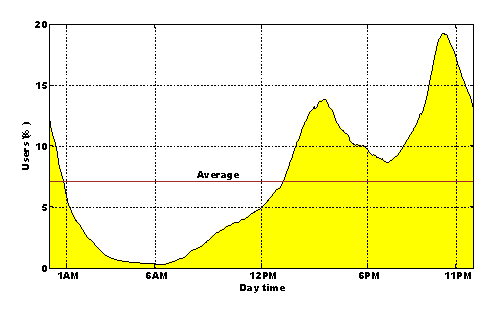
\includegraphics{image/chart3.eps}}}
	\caption{User activity of the IPTV service~\cite{DBLP:conf/conext/ValanciusLMDR09}}.
	\label{fig:iptv}
	\normalsize
\end{figure}

Therefore, to make a nano data center platform energy-efficient,
it is necessary to increase the active time ratio.
From our view,
a possible solution is to turn off the nano server time to time to reduce the idle time of the nano servers.
But for the nano servers attached to DSL-modems or other functional devices,
such as the NaDa model proposed in~\cite{DBLP:conf/conext/ValanciusLMDR09},
turning off nano servers can lead to side-effects on the usage of other internet services of users,
and thus the implementation of this solution requires further study.
Another possible solution is to modify the applications for the nano data center,
such as running multiple applications that have different peak hours,
aiming to maximize the active time of the nano servers.
So far we are unaware of any research tackling these problems,
and thus we list the activation of nano servers as one of the four technical challenges towards nano data center development.

\subsubsection{Access Network}

As discussed in Section~\ref{sec:model}, the access network connects nano servers to the edge network.
According to the analysis proposed in~\cite{tradeoff} and~\cite{DBLP:journals/sigmetrics/JalaliAVHAT14},
the power consumption of the access network needs to be counted twice for nano data centers,
i.e. $E_\text{access}$ needs to be counted both in $E_\text{req}$ and $E_\text{serv}$.
Thus, the energy efficiency of the access network has a large impact on the energy efficiency of the nano data center platform.

The energy consumption of the access network has been studied in~\cite{DBLP:journals/sigmetrics/JalaliAVHAT14} and~\cite{accessNetwork}.
Both studies refer Passive Optical Networks (PON) as energy-efficient access networks,
and indicate that wireless networks (WiMAX~\cite{accessNetwork}, 4G, WiFi~\cite{DBLP:journals/sigmetrics/JalaliAVHAT14} are relatively energy-inefficient.
Figure~\ref{fig:accessNet} shows a comparison of energy consumption between nano data centers using different access networks and centralized data centers with different energy consumption values,
where the curves for GPON and Ethernet almost overlap, and the curves for WiFi and centralized data center with 20$\mu J/$bit almost overlap.
We can see that different access networks result in huge difference of energy consumption,
and nano data centers attached to energy-inefficient access networks consume even more energy than centralized data centers.
 
\begin{figure}[h]
	\fontsize{12}{12} \selectfont
	\centerline{\resizebox{5cm}{!}{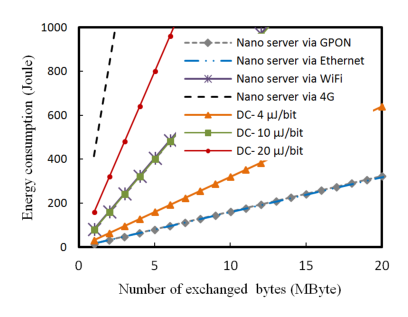
\includegraphics{image/chart.eps}}}
	\caption{A comparison of energy consumption between nano data centers using different access networks and centralized data centers with different energy consumption values~\cite{DBLP:conf/conext/ValanciusLMDR09}}.
	\label{fig:accessNet}
	\normalsize
\end{figure}

For nano data centers,
since each nano servers is possessed by an end-user,
it requires further study on the access network that these end-users may or may not use,
before one can determine whether the implementation of nano data centers can save energy or not.

Another concern regarding the access network of nano data centers is the trade-off between energy consumption and the access rate.  
Figure~\ref{fig:accessNet2} shows their correlation from two aspects.
As shown in the left figure,
for a single user,
the power consumption increases with the average access rate,
and as shown in the right figure, 
the energy per bit decreases with the average access rate.
For the two relatively energy-efficient access networks -- Point-to-Point optical access network (PtP) and PON,
their performance show different trends with the increase of the access rate.
While PON is more energy efficient for a low access rate,
it consumes more energy than PtP when the access rate surpasses 300Mb/s.
Thus, it also requires further study on the selection of the access networks with respect to the expected access rate.

\begin{figure}[h]
	\fontsize{12}{12} \selectfont
	\centerline{\resizebox{14cm}{!}{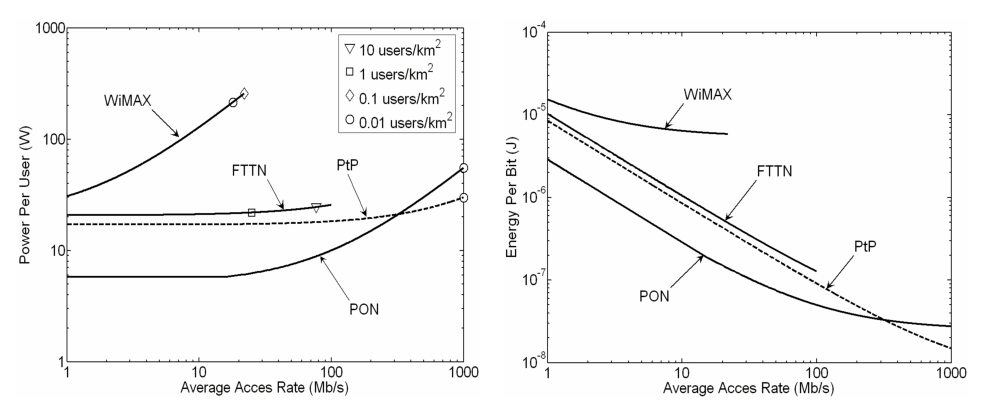
\includegraphics{image/chart4.eps}}}
	\caption{Power consumption per user for different access networks and energy per bit of different access networks~\cite{accessNetwork}}.
	\label{fig:accessNet2}
	\normalsize
\end{figure}

\subsubsection{Trade-off: Distance and Replication}

The energy consumption of the data transmission process ($E_\text{trans}$) in nano data center platforms is dependent on the number of hops in the edge ($h_\text{edge}$) and core networks ($h_\text{core}$),
as mentioned in (\ref{eq:trans}) in Section~\ref{sec:model}.
\cite{DBLP:journals/sigmetrics/JalaliAVHAT14} estimated the average number of hops in the edge and core networks to be $3$ and $5$,
using \textit{traceroute} from end-user devices to WordPress~\cite{wordpress} servers.
The number of these hops can be understood as the distance between the end-user requesting data and the end-user hosting the corresponding data.
Regarding the location of the communicating end-users,
the number of hops shows large variation:
for non-local users,
\cite{DBLP:journals/sigmetrics/JalaliAVHAT14} measured $h_\text{edge}$ and $h_ \text{core}$ as $3$ and $8$;
and for local users,
$h_\text{edge}$ and $h_\text{core}$ are measured as $1$ and $2$.
Figure~\ref{fig:location} shows the energy consumption of the the core and edge networks for the data transmission between local and non-local users,
and compares them with the centralized data center.
We can see that if an end-user accesses data from a non-local nano server, 
the energy consumption of the edge and core networks can be even higher than accessing data from a centralized data center.

\begin{figure}[h]
	\fontsize{12}{12} \selectfont
	\centerline{\resizebox{5cm}{!}{\input{image/chart5.eps_tex}}}
	\caption{Energy consumption of core and edge networks for accesing data from different locations~\cite{DBLP:journals/sigmetrics/JalaliAVHAT14}}
	\label{fig:location}
	\normalsize
\end{figure}

A natural solution to reduce or balance the data transmission distance is to add data replicas~\cite{tradeoff}~\cite{iptv}.
However,
while data replication can be beneficial to the energy-efficiency in the transmission process,
it also leads to the increase of the energy consumption for storing the data.
\cite{iptv} indicated that the data replication strategy should depend on the popularity of the data.
Figure~\ref{fig:popularity} shows the contribution of storage, servers and transmission to the total power consumption of IPTV services,
where 20 replicas of a 2-hour SD movie are stored in 20 different data centers~\cite{iptv}. 
We can see that the storage cost dominates the total energy consumption when the movie is rarely downloaded,
and the transmission cost becomes significant as the data popularity increases. 
Regarding this,
for movies that are frequently downloaded,
it is more energy-efficient to keep a relatively large number of replicas to reduce the energy consumption in the transmission process;
and for movies that are rarely downloaded,
it is more energy-efficient to keep a relatively small number of replicas to reduce the energy consumption in the storage.

\begin{figure}[h]
	\fontsize{12}{12} \selectfont
	\centerline{\resizebox{5cm}{!}{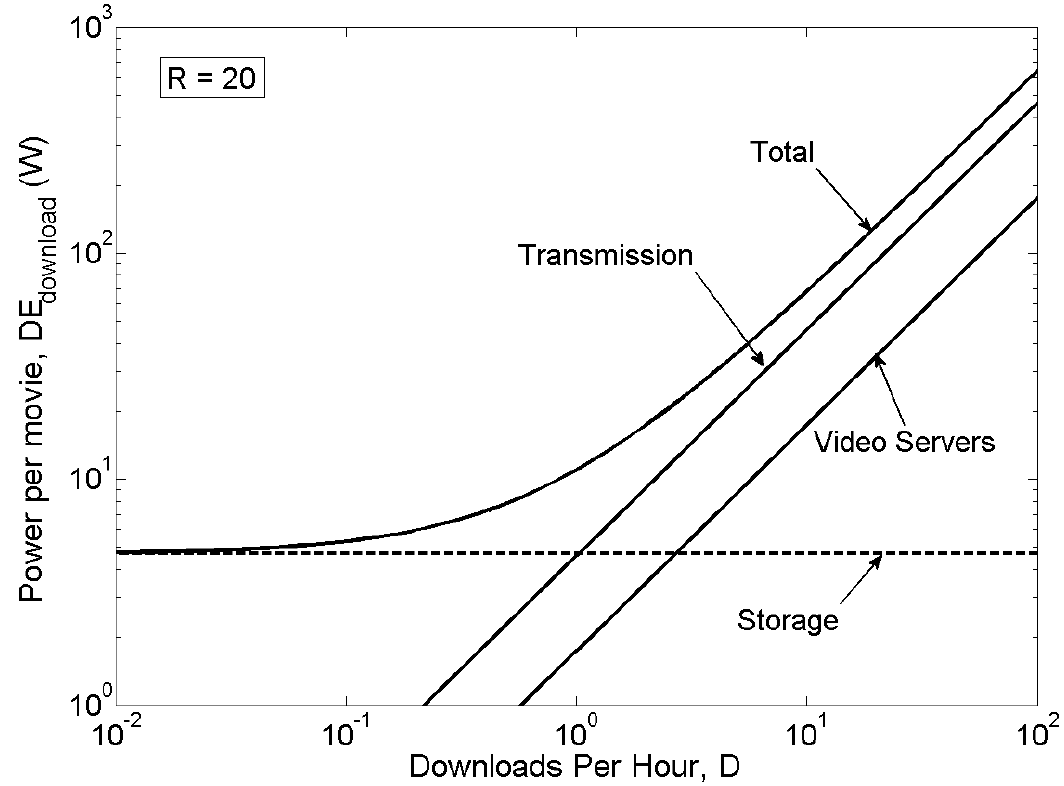
\includegraphics{image/chart7.png}}}
	\caption{The contribution of storage, servers and transmission to the total power consumption of IPTV services with respect to data popularity~\cite{iptv}}.
	\label{fig:popularity}
	\normalsize
\end{figure}

\cite{tradeoff} compared the energy consumption for downloading movies from nano data centers and from centralized data centers with respect to the access frequency,
under the scenario that a centralized data centers keeps two replicas of each data,
and nano data centers keeps 2, or 10, or 100 replicas of each data.
The result indicated that a centralized data center is more efficient than nano data centers for unpopular data.

Thus,
we regard finding the balance between the transmission distance and the number of replicas as one the technical challenges towards the development of nano data centers.
From our view,
a possible solution is to detect the popularity of each individual data dynamically,
and adjusting the number of replicas for each data accordingly.
However,
further study on the negotiation and configuration mechanism is required.









\section{Evaluation/Results}
% Describe your evaluation methodology and present results and analyses
%includes research results and interview results etc.; includes Achievements
We collect all challenges that we figured out in the section \ref{sec:challenges} and put them into political, legal and technical issues. In table \ref{tab:summary} we can see the summary of all challenges that we have established in our research. 

\begin{table}
\begin{minipage}{\columnwidth}
\begin{center}
\begin{tabular}{lll}
\toprule
Political issues & Legal issues & Technical issues \\
\hline
\parbox{.3\linewidth}{Distribution of data between ISP: including international partnerships with political policies} & \parbox{.3\linewidth}{Data Protection of the EU (GDPR)} & 
\parbox[c][2cm]{.3\linewidth}{Activation time: maximize the active time of nano serves, and avoid a large idle time, to get a hight ratio} \\


\parbox{.3\linewidth}{Net neutrality: conflict of interest, if ISP would also providing data} & 
\parbox{.3\linewidth}{Liability of stored data in the nano server} & 
\parbox[c][2.5cm]{.3\linewidth}{Access network: futher study on the access network that the end-user use, also on the selection of the access network, depending on the access rate} \\


\parbox{.3\linewidth}{} & 
\parbox{.3\linewidth}{} & 
\parbox[c][1.5cm]{.3\linewidth}{Trade-off: Distance: finding balance between the transmission distance} \\

\parbox{.3\linewidth}{} & 
\parbox{.3\linewidth}{} & 
\parbox[c][1.5cm]{.3\linewidth}{Trade-off: Replication: finding a well-chosen number of data replicas} \\				
\bottomrule
\end{tabular}
\end{center}
\bigskip\centering
\end{minipage}
\caption{Summary of all challenges towards a nano data center platfrom, categorized by political, legal and technical issues}\label{tab:summary}
\end{table}

As we can see, there are more technical challenges on one hand, and a few challenges in political and legal categories on the other. Nevertheless, we would not underestimate these non-technical challenges, because this is a rough estimate in this field. Furthermore, as we have 
above-mentioned, these issues will give just an overview. For more 
detailed analysis, there a further studies required.

\section{Discussion}
% What do we have, what do the others have in their paper?

% What lessons are lerned and what goals are achieved in the project

In our paper we analyses the multiple challenges towards nano data center development. There are a few papers about that approach as a  green alternative or addition to monolithic data centers. These works includes the technical and non-technical issues towards these nano servers. But nowadays, we haven't had any nano data center platform in practical use. In our research we are figuring out the challenges towards the implementation of such a platform.


\section{Conclusion and Future Work}
%inclde idea: use onliney surveys to invite experts to answer questions
In section \ref{sec:challenges} we can see that is isn't as easy as accepted in \cite{Laoutaris:2008:EEC:1341431.1341442} or other works to implement a nano data platform. There are a further more steps to put this in practice. Some issues which still have to investigate and to researched in more detail. In our work we figured out the main challenges for the next steps towards a common use of nano date server.
%future work
For next steps there are more studies required in in technical and non-technical challenges. There are probably more political and legal challenges than we  have considered in our work. This is also specifically related to the geographic location and the local  dispensation of justice.

In \ref{sec:model} we have defined the technical challenges. These require in part further investigations.
On the one hand, this concerns a further investigation of a well-chosen activity time of the nano server in order to achieve better energy efficiency.
Further detailed research is also needed for the selection of access networks to investigate which network is more suitable.
Finally, another investigation is needed to find a good balance between the transmission distance and the number of data replicas.




% Bibliography
\bibliographystyle{ACM-Reference-Format}
\bibliography{sample-bibliography}

% Appendix
\appendix
\section{Questionnaire}
\begin{enumerate}
\label{appendix:quest}
\item On the website of the LRZ it can be read that \textit{Green IT} is important \cite{LRZGreenIT}. What has been achieved or improved so far?
\item In 2012, the LRZ was awarded the German Data Center Award for \textit{energy and resource efficient data centers} \cite{LRZGreenIT}. What makes the LRZ better on \textit{Green IT} than other data centers?
\item What does the LRZ offer its customers? Are there any special \textit{Green IT} services available? Does the customer have an influence on more environmentally conscious use?
\item Today's use of Internet services has changed massively \cite{TheZetta68:online}. How has the LRZ adapted accordingly?
\item Why are the big data centers still so popular? What are the reasons/advantages? Are these political, economic or technical?
\item Are there any disadvantages with monolithic data centers?
\item Have you heard of an alternative solution to monolithic data centers? There are, among others, some research on nano data centers. Does the LRZ also work with these approaches? What is your opinion?
\item In your opinion, what are the advantages and disadvantages of nano data centers?
\item How does the LRZ see the data centers of the future? What could be possible? Is it realistic that monolithic data centers could be replaced by special peer-to-peer networks?
\item Do you think there are any difficulties or special challenges that need to be solved in order to implement nano data centers suitable for the mass or as new state of the art? What are the difficulties oder challenges in your opinion?
\item Do you have any idea or approach how to solve these difficulties or challenges?
\item Would you have an idea for other alternative systems?
\end{enumerate}



\end{document}
